% report.tex - Frontpage for the report (place in Report/)
\documentclass[a4paper,12pt]{article}
\usepackage[utf8]{inputenc}
\usepackage[T1]{fontenc}
\usepackage{graphicx}
\usepackage{eso-pic}
\usepackage[HTML]{xcolor}
\usepackage{tikz}
\usepackage{geometry}
\usepackage{parskip}
\usepackage{setspace}
\usepackage{caption}
\usepackage{subcaption}
\usepackage{float}
\usepackage{gensymb}
\usepackage{ulem}
\usepackage{amsmath}
\usepackage{amsfonts}
\usepackage{microtype}
\usepackage{geometry}
\usepackage{setspace}
\usepackage{tabularx}
\usepackage{longtable}
\usepackage{booktabs}
\usepackage{hyperref}
\usepackage{makecell}
\usepackage[
backend=biber,
style=alphabetic,
sorting=ynt
]{biblatex}
\addbibresource{bibliography/bibliography.bib}

\geometry{margin=2.5cm}

\AddToShipoutPictureBG{
  \definecolor{sidebar}{HTML}{008571}
  \begin{tikzpicture}[remember picture,overlay]
    \fill[sidebar]
    (current page.north west)
    rectangle
    ([xshift=1.2cm]current page.south west);
  \end{tikzpicture}
}

\begin{document}
\begin{titlepage}
    \thispagestyle{empty}
    \centering
    \vspace*{2cm}

    % Logos at the corners
    \begin{figure}[t]
        \centering
        
\includegraphics[width=0.6\textwidth]{logos/nmbu_logo_tekst.jpeg}
    \end{figure}
    %\includegraphics[width=0.35\textwidth]{logos/eik_lab_logo.jpeg}\\[1.5cm]

    {\Huge\bfseries TEL200 - Introduction to Robotics}\\[0.5cm]
    {\Large\itshape Group 5}\\[1.5cm]
    \begin{figure}[H]
        \centering
        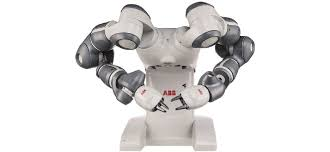
\includegraphics[width=.7\textwidth]{images/yumi.jpeg}
    \end{figure}
    {\Large\itshape Yumi Lab Project}\\[1.5cm]

    \rule{0.6\textwidth}{1pt}\\[0.8cm]

    {\Large\bfseries Authors}\\[0.3cm]
    {\large Andreas Brustad \\ Johannes Standal \\ Håkon Bekken}\\[1cm]

    %{\large\bfseries Supervisor}\\[0.3cm]
    %{\large Dr. Supervisor Name}\\[2cm]

    {}

    \vfill

    \small Norwegian University of Life Sciences
\end{titlepage}

% NMBU watermark
\AddToShipoutPictureBG{%
  \AtPageUpperLeft{%
    \raisebox{-3.5cm}{%
      \hspace{1.07\textwidth}%
      
\includegraphics[width=3cm]{logos/nmbu_logo.png}
    }%
  }%
}

\tableofcontents

\newpage

\section{Abstract}

\newpage

\section{Introduction}

\newpage

\section{Method}
\subsection{RS BASIC}

\subsection{YuMi Appliction}

The control software for the dual-arm YuMi robot (IRB 14000) was developed in ABB's RAPID programming language within RobotStudio. The program implements a modular pick-and-place application that handles three distinct geometric objects (cube, cylinder, and triangular prism) based on external digital input signals. A key safety and recovery feature is the interrupt-driven emergency stop handling.

The main structure is defined in \texttt{MODULE Module1}. A large number of \texttt{CONST robtarget} declarations define the taught positions for safe approach points, alignment poses, gripping locations, and drop-off positions for each object and work object (\texttt{cube}, \texttt{cyl}, \texttt{prizm}). These targets were recorded using the FlexPendant or RobotStudio's teaching interface and include full pose information (position, orientation quaternion, configuration data, and external axes).

The entry point is the \texttt{Main()} procedure, which first initializes the gripper system via \texttt{g\_Init}. To prevent multiple connections of the same interrupt variable (a common source of runtime errors \texttt{ERR\_ALRDYCNT}), an initialization guard is used:

\begin{verbatim}
IF NOT interrupts_setup THEN
    SkipWarn;
    CONNECT stop_emer WITH EmergencyStop;
    ISignalDI di_EmergencySituation, high, stop_emer;
    interrupts_setup := TRUE;
ENDIF
\end{verbatim}

A continuous loop then polls three digital input signals (\texttt{di\_cube}, \texttt{di\_cylinder}, \texttt{di\_prism}) and calls the corresponding path procedure when the respective signal is high:

\begin{verbatim}
WHILE TRUE DO
    IF DInput(di_cube) = 1 THEN CubePath;
    ELSEIF DInput(di_cylinder) = 1 THEN CyliPath;
    ELSEIF DInput(di_prism) = 1 THEN PrizmPath;
    ENDIF
    WaitTime 0.1;
ENDWHILE
\end{verbatim}

Each path procedure (\texttt{CubePath}, \texttt{CyliPath}, \texttt{PrizmPath}) consists of a sequence of \texttt{MoveJ} instructions with velocity \texttt{v500}, zone \texttt{fine} or \texttt{z100}, and the appropriate work object. The motion sequence follows a typical pick-and-place pattern: move to approach pose $\to$ align above object $\to$ descend to grip $\to$ grip object $\to$ lift $\to$ transport to drop position $\to$ release $\to$ return to home. Gripper commands (\texttt{g\_GripIn}, \texttt{g\_GripOut}) are inserted at the appropriate points, and short \texttt{WaitTime} instructions ensure stable execution and allow time for gripper action.

The emergency stop functionality is implemented via a trap routine triggered by the rising edge of the digital input \texttt{di\_EmergencySituation}:

\begin{verbatim}
TRAP EmergencyStop
    SkipWarn;
    StopMove;
    WaitUntil di_EmergencySituation = 0;
    StorePath;
    IF DInput(di_home) = 1 THEN
        ClearPath;
        MoveJ RealHome, v500, z100, Servo\WObj:=wobj0;
        WaitTime 1;
        ExitCycle;
    ELSE
        RestoPath;
        StartMove;
    ENDIF
ENDTRAP
\end{verbatim}

When the emergency signal is active, the robot immediately halts motion (\texttt{StopMove}). After the signal is released, the program checks \texttt{di\_home}. If high, the path context is cleared, the robot moves to a safe recovery pose (\texttt{RealHome}), and \texttt{ExitCycle} resets execution to the beginning of the \texttt{Main} procedure (requiring continuous run mode in the controller). Otherwise, the original interrupted path is restored and motion resumes from the point of interruption.

This interrupt-based architecture ensures robust safety handling while maintaining deterministic cyclic behavior in normal operation. All motion commands use joint interpolation (\texttt{MoveJ}) to avoid singularities and provide predictable behavior during teaching and execution.

\newpage

\section{Results}

\newpage

\section{Discussion}

\newpage

\section{Conclusions}

\newpage

\section{Bibliography}
\printbibliography

\end{document}